%---------------
%╔═╗╔═╗╔╦╗╦ ╦╔═╗
%╚═╗║╣  ║ ║ ║╠═╝
%╚═╝╚═╝ ╩ ╚═╝╩  
%---------------

% language setup
\newcommand{\docLanguage}{ngerman}
%\newcommand{\docLanguage}{english}

% DOCUMENT SETUP
\documentclass[12pt, oneside, a4paper, \docLanguage]{report}
\usepackage[left=3cm, 
			right=2.5cm, 
			top=2.5cm, 
			bottom=2.5cm, 
			includehead, 
			includefoot]{geometry}

% line spacing
\usepackage{setspace}
\setstretch{1,25} % 15/12 --> 1.25

% encoding setup
% T1 font encoding for languages that use a latin alphabet
\usepackage[T1]{fontenc} 

% enhanced input encoding handling - utf8 for äÄüÜöÖß...
\usepackage[utf8]{inputenc}

%de­fines Adobe Times Ro­man as de­fault text font
\usepackage{mathptmx}
\usepackage{times} % needed for acronym package

%PDF linking package
\usepackage[hidelinks]{hyperref}


% Language Setup
\usepackage[\docLanguage]{babel}
% after babel - set chapter string
\AtBeginDocument{\renewcommand{\chaptername}{}}

% language specific bibliography style
\usepackage[numbers, square]{natbib}
%\setcitestyle{square,aysep={},yysep={;}}
\usepackage[fixlanguage]{babelbib}
\selectbiblanguage{\docLanguage}
% bliographystyle setup
% babel specific: babplain, babplai3, babalpha, babunsrt, bababbrv, bababbr3
\bibliographystyle{babunsrt}


% enumeration
\usepackage{enumitem}
% tabular extension tabularx
\usepackage{tabularx}

% math packages
\usepackage{amsmath}
\usepackage{nicefrac}
\usepackage{amsthm}
\usepackage{amsbsy}
\usepackage{amssymb}
\usepackage{amsfonts}
%\usepackage{MnSymbol}


%special characters
\usepackage{amssymb}
\usepackage{upgreek,textgreek}

% acronym package
\usepackage[printonlyused, footnote]{acronym}

% breakable text in \seqsplit{}
\usepackage{seqsplit}

% \textmu
\usepackage{textcomp}

% package provides a way to compile sections of a document using the same preamble as the main document
\usepackage{subfiles}

% driver-independent color extension - used by listings,tabularx
\usepackage[usenames,dvipsnames,table,xcdraw]{xcolor}

% -- SYNTAX HIGHLIGHTING --
\usepackage{listings}
%% bash command line Syntax Highlighting
\lstdefinestyle{BASH_CMD}{ 
  columns=fullflexible,            % copy pasteable listings
  language=bash,
  basicstyle=\small\sffamily,
  basicstyle   = \small \ttfamily,
  keywordstyle = [1]\small \ttfamily,
  keywordstyle = [2]\small \ttfamily,
  commentstyle = \small \ttfamily,
  numbers=none,
  captionpos=b, 
  breaklines=true,
  numberstyle=\tiny,
  numbersep=3pt,
  frame=tlrb,
  columns=fullflexible,
  backgroundcolor=\color{white!20},
  linewidth=\linewidth,
  literate=                        % replace in code
     {Ö}{{\"O}}1 
     {Ä}{{\"A}}1 
     {Ü}{{\"U}}1 
     {ß}{{\ss}}2 
     {ü}{{\"u}}1 
     {ä}{{\"a}}1 
     {ö}{{\"o}}1 
     {â}{{\^{a}}}1 
     {Â}{{\^{A}}}1 
     {ç}{{\c{c}}}1 
     {Ç}{{\c{C}}}1 
     {ğ}{{\u{g}}}1 
     {Ğ}{{\u{G}}}1 
     {ı}{{\i}}1 
     {İ}{{\.{I}}}1 
     {ş}{{\c{s}}}1 
     {Ş}{{\c{S}}}1 
}
 % adds style BASH_CMD
%% Matlab Syntax Highlighting
\colorlet{keyword}{blue!100!black!80}
\colorlet{STD}{Lavender}
\colorlet{comment}{green!90!black!90}
\definecolor{mygreen}{rgb}{0,0.6,0}
\definecolor{mygray}{rgb}{0.5,0.5,0.5}
\definecolor{mymauve}{rgb}{0.58,0,0.82}


\lstdefinestyle{BASH_SCRIPT}{ 
  language     = bash,
  basicstyle   = \footnotesize \ttfamily,
  keywordstyle = [1]\color{keyword}\bfseries,
  keywordstyle = [2]\color{STD}\bfseries,
  commentstyle = \color{mygreen}\itshape,
  backgroundcolor=\color{white},   % choose the background color; you must add \usepackage{color} 
  columns=fullflexible,            % copy pasteable listings
                                   % or \usepackage{xcolor}
  basicstyle=\footnotesize,        % the size of the fonts that are used for the code
  breakatwhitespace=false,         % sets if automatic breaks should only happen at whitespace
  breaklines=true,                 % sets automatic line breaking
  captionpos=b,                    % sets the caption-position to bottom
  extendedchars=true,              % lets you use non-ASCII characters; for 8-bits encodings only,
                                   % does not work with UTF-8
  frame=single,                    % adds a frame around the code
  keepspaces=true,                 % keeps spaces in text, useful for keeping indentation of code
                                   % (possibly needs columns=flexible)
  numbers=left,                    % where to put the line-numbers; possible values are 
                                   % (none, left, right)
  numbersep=5pt,                   % how far the line-numbers are from the code
  numberstyle=\tiny\color{mygray}, % the style that is used for the line-numbers
  rulecolor=\color{black},         % if not set, the frame-color may be changed on line-breaks
                                   % within not-black text (e.g. comments (green here))
  showspaces=false,                % show spaces everywhere adding particular underscores; it
  	                               % overrides 'showstringspaces'
  showstringspaces=false,          % underline spaces within strings only
  showtabs=false,                  % show tabs within strings adding particular underscores
  stepnumber=1,                    % the step between two line-numbers. If it's 1, each line 
                                   % will be numbered
  stringstyle=\color{mymauve},     % string literal style
  tabsize=2,                       % sets default tabsize to 2 spaces
  title=\lstname,                  % set title name
  literate=                        % replace in code
     {Ö}{{\"O}}1 
     {Ä}{{\"A}}1 
     {Ü}{{\"U}}1 
     {ß}{{\ss}}2 
     {ü}{{\"u}}1 
     {ä}{{\"a}}1 
     {ö}{{\"o}}1 
     {â}{{\^{a}}}1 
     {Â}{{\^{A}}}1 
     {ç}{{\c{c}}}1 
     {Ç}{{\c{C}}}1 
     {ğ}{{\u{g}}}1 
     {Ğ}{{\u{G}}}1 
     {ı}{{\i}}1 
     {İ}{{\.{I}}}1 
     {ş}{{\c{s}}}1 
     {Ş}{{\c{S}}}1 
} % adds style BASH_SCRIPT
% Matlab Syntax Highlighting
\colorlet{keyword}{blue!100!black!80}
\colorlet{STD}{red}
\colorlet{comment}{green!90!black!90}
\definecolor{mygreen}{rgb}{0,0.6,0}
\definecolor{mygray}{rgb}{0.5,0.5,0.5}
\definecolor{mymauve}{rgb}{0.58,0,0.82}


\lstdefinestyle{LATEX}{ 
  language     = [LaTeX]{TeX},
  basicstyle   = \footnotesize \ttfamily,
  keywordstyle = [1]\color{keyword}\bfseries,
  keywordstyle = [2]\color{comment}\bfseries,
  commentstyle = \color{mygray}\itshape,
  %backgroundcolor=\color{white},   % choose the background color; you must add \usepackage{color} 
                                   % or \usepackage{xcolor}
  basicstyle=\footnotesize,        		   % the size of the fonts that are used for the code
  breakatwhitespace=false,         % sets if automatic breaks should only happen at whitespace
  columns=fullflexible,            % copy pasteable listings
  breaklines=true,                 % sets automatic line breaking
  captionpos=c,                    % sets the caption-position to bottom
  extendedchars=true,              % lets you use non-ASCII characters; for 8-bits encodings only,
                                   % does not work with UTF-8
  frame=single,                    % adds a frame around the code
  keepspaces=true,                 % keeps spaces in text, useful for keeping indentation of code
                                   % (possibly needs columns=flexible)
  numbers=left,                    % where to put the line-numbers; possible values are 
                                   % (none, left, right)
  numbersep=4pt,                   % how far the line-numbers are from the code
  numberstyle=\tiny\color{mygray}, % the style that is used for the line-numbers
  rulecolor=\color{black},         % if not set, the frame-color may be changed on line-breaks
                                   % within not-black text (e.g. comments (green here))
  showspaces=false,                % show spaces everywhere adding particular underscores; it
  	                               % overrides 'showstringspaces'
  showstringspaces=false,          % underline spaces within strings only
  showtabs=false,                  % show tabs within strings adding particular underscores
  stepnumber=1,                    % the step between two line-numbers. If it's 1, each line 
                                   % will be numbered
  stringstyle=\color{mymauve},     % string literal style
  tabsize=2,                       % sets default tabsize to 2 spaces
  title=\lstname,                  % set title name
  literate=                        % replace in code
     {Ö}{{\"O}}1 
     {Ä}{{\"A}}1 
     {Ü}{{\"U}}1 
     {ß}{{\ss}}2 
     {ü}{{\"u}}1 
     {ä}{{\"a}}1 
     {ö}{{\"o}}1 
     {â}{{\^{a}}}1 
     {Â}{{\^{A}}}1 
     {ç}{{\c{c}}}1 
     {Ç}{{\c{C}}}1 
     {ğ}{{\u{g}}}1 
     {Ğ}{{\u{G}}}1 
     {ı}{{\i}}1 
     {İ}{{\.{I}}}1 
     {ş}{{\c{s}}}1 
     {Ş}{{\c{S}}}1 
} % adds style LATEX
%% Matlab Syntax Highlighting
\colorlet{keyword}{blue!100!black!80}
\colorlet{STD}{Lavender}
\colorlet{comment}{green!90!black!90}
\definecolor{mygreen}{rgb}{0,0.6,0}
\definecolor{mygray}{rgb}{0.5,0.5,0.5}
\definecolor{mymauve}{rgb}{0.58,0,0.82}


\lstdefinestyle{MATLAB}{ 
  language     = Matlab,
  basicstyle   = \footnotesize \ttfamily,
  keywordstyle = [1]\color{keyword}\bfseries,
  keywordstyle = [2]\color{STD}\bfseries,
  commentstyle = \color{mygreen}\itshape,
  backgroundcolor=\color{white},   % choose the background color; you must add \usepackage{color} 
                                   % or \usepackage{xcolor}
  basicstyle=\footnotesize,        % the size of the fonts that are used for the code
  breakatwhitespace=false,         % sets if automatic breaks should only happen at whitespace
  columns=fullflexible,            % copy pasteable listings
  breaklines=false,                % sets automatic line breaking
  captionpos=c,                    % sets the caption-position to bottom
  extendedchars=true,              % lets you use non-ASCII characters; for 8-bits encodings only,
                                   % does not work with UTF-8
  frame=single,                    % adds a frame around the code
  keepspaces=true,                 % keeps spaces in text, useful for keeping indentation of code
                                   % (possibly needs columns=flexible)
  numbers=left,                    % where to put the line-numbers; possible values are 
                                   % (none, left, right)
  numbersep=5pt,                   % how far the line-numbers are from the code
  numberstyle=\tiny\color{mygray}, % the style that is used for the line-numbers
  rulecolor=\color{black},         % if not set, the frame-color may be changed on line-breaks
                                   % within not-black text (e.g. comments (green here))
  showspaces=false,                % show spaces everywhere adding particular underscores; it
  	                               % overrides 'showstringspaces'
  showstringspaces=false,          % underline spaces within strings only
  showtabs=false,                  % show tabs within strings adding particular underscores
  stepnumber=1,                    % the step between two line-numbers. If it's 1, each line 
                                   % will be numbered
  stringstyle=\color{mymauve},     % string literal style
  tabsize=2,                       % sets default tabsize to 2 spaces
  title=\lstname,                  % set title name
  literate=                        % replace in code
     {Ö}{{\"O}}1 
     {Ä}{{\"A}}1 
     {Ü}{{\"U}}1 
     {ß}{{\ss}}2 
     {ü}{{\"u}}1 
     {ä}{{\"a}}1 
     {ö}{{\"o}}1 
     {â}{{\^{a}}}1 
     {Â}{{\^{A}}}1 
     {ç}{{\c{c}}}1 
     {Ç}{{\c{C}}}1 
     {ğ}{{\u{g}}}1 
     {Ğ}{{\u{G}}}1 
     {ı}{{\i}}1 
     {İ}{{\.{I}}}1 
     {ş}{{\c{s}}}1 
     {Ş}{{\c{S}}}1 
} % adds style MATLAB
% Matlab Syntax Highlighting
\colorlet{keyword}{blue!100!black!80}
\colorlet{STD}{Lavender}
\colorlet{comment}{green!90!black!90}
\definecolor{mygreen}{rgb}{0,0.6,0}
\definecolor{mygray}{rgb}{0.5,0.5,0.5}
\definecolor{mymauve}{rgb}{0.58,0,0.82}


\lstdefinestyle{PYTHON}{ 
  language     = Python,
  basicstyle   = \footnotesize \ttfamily,
  keywordstyle = [1]\color{keyword}\bfseries,
  keywordstyle = [2]\color{STD}\bfseries,
  commentstyle = \color{mygreen}\itshape,
  backgroundcolor=\color{white},   % choose the background color; you must add \usepackage{color} 
                                   % or \usepackage{xcolor}
  basicstyle=\footnotesize,        % the size of the fonts that are used for the code
  columns=fullflexible,            % copy pasteable listings
  breakatwhitespace=false,         % sets if automatic breaks should only happen at whitespace
  breaklines=false,                % sets automatic line breaking
  captionpos=c,                    % sets the caption-position to bottom
  extendedchars=true,              % lets you use non-ASCII characters; for 8-bits encodings only,
                                   % does not work with UTF-8
  frame=single,                    % adds a frame around the code
  keepspaces=true,                 % keeps spaces in text, useful for keeping indentation of code
                                   % (possibly needs columns=flexible)
  numbers=left,                    % where to put the line-numbers; possible values are 
                                   % (none, left, right)
  numbersep=5pt,                   % how far the line-numbers are from the code
  numberstyle=\tiny\color{mygray}, % the style that is used for the line-numbers
  rulecolor=\color{black},         % if not set, the frame-color may be changed on line-breaks
                                   % within not-black text (e.g. comments (green here))
  showspaces=false,                % show spaces everywhere adding particular underscores; it
  	                               % overrides 'showstringspaces'
  showstringspaces=false,          % underline spaces within strings only
  showtabs=false,                  % show tabs within strings adding particular underscores
  stepnumber=1,                    % the step between two line-numbers. If it's 1, each line 
                                   % will be numbered
  stringstyle=\color{mymauve},     % string literal style
  tabsize=2,                       % sets default tabsize to 2 spaces
  title=\lstname,                  % set title name
  literate=                        % replace in code
     {Ö}{{\"O}}1 
     {Ä}{{\"A}}1 
     {Ü}{{\"U}}1 
     {ß}{{\ss}}2 
     {ü}{{\"u}}1 
     {ä}{{\"a}}1 
     {ö}{{\"o}}1 
     {â}{{\^{a}}}1 
     {Â}{{\^{A}}}1 
     {ç}{{\c{c}}}1 
     {Ç}{{\c{C}}}1 
     {ğ}{{\u{g}}}1 
     {Ğ}{{\u{G}}}1 
     {ı}{{\i}}1 
     {İ}{{\.{I}}}1 
     {ş}{{\c{s}}}1 
     {Ş}{{\c{S}}}1 
} % adds style PYTHON
%% Matlab Syntax Highlighting
\colorlet{keyword}{blue!100!black!80}
\colorlet{STD}{Lavender}
\colorlet{comment}{green!90!black!90}
\definecolor{mygreen}{rgb}{0,0.6,0}
\definecolor{mygray}{rgb}{0.5,0.5,0.5}
\definecolor{mymauve}{rgb}{0.58,0,0.82}


\lstdefinestyle{CPP}{ 
  language     = C++,
  basicstyle   = \footnotesize \ttfamily,
  keywordstyle = [1]\color{keyword}\bfseries,
  keywordstyle = [2]\color{STD}\bfseries,
  commentstyle = \color{mygreen}\itshape,
  backgroundcolor=\color{white},   % choose the background color; you must add \usepackage{color} 
                                   % or \usepackage{xcolor}
  columns=fullflexible,            % copy pasteable listings
  basicstyle=\footnotesize,        % the size of the fonts that are used for the code
  breakatwhitespace=false,         % sets if automatic breaks should only happen at whitespace
  breaklines=false,                % sets automatic line breaking
  captionpos=c,                    % sets the caption-position to bottom
  extendedchars=true,              % lets you use non-ASCII characters; for 8-bits encodings only,
                                   % does not work with UTF-8
  frame=single,                    % adds a frame around the code
  keepspaces=true,                 % keeps spaces in text, useful for keeping indentation of code
                                   % (possibly needs columns=flexible)
  numbers=left,                    % where to put the line-numbers; possible values are 
                                   % (none, left, right)
  numbersep=5pt,                   % how far the line-numbers are from the code
  numberstyle=\tiny\color{mygray}, % the style that is used for the line-numbers
  rulecolor=\color{black},         % if not set, the frame-color may be changed on line-breaks
                                   % within not-black text (e.g. comments (green here))
  showspaces=false,                % show spaces everywhere adding particular underscores; it
  	                               % overrides 'showstringspaces'
  showstringspaces=false,          % underline spaces within strings only
  showtabs=false,                  % show tabs within strings adding particular underscores
  stepnumber=1,                    % the step between two line-numbers. If it's 1, each line 
                                   % will be numbered
  stringstyle=\color{mymauve},     % string literal style
  tabsize=2,                       % sets default tabsize to 2 spaces
  title=\lstname,                  % set title name
  literate=                        % replace in code
     {Ö}{{\"O}}1 
     {Ä}{{\"A}}1 
     {Ü}{{\"U}}1 
     {ß}{{\ss}}2 
     {ü}{{\"u}}1 
     {ä}{{\"a}}1 
     {ö}{{\"o}}1 
     {â}{{\^{a}}}1 
     {Â}{{\^{A}}}1 
     {ç}{{\c{c}}}1 
     {Ç}{{\c{C}}}1 
     {ğ}{{\u{g}}}1 
     {Ğ}{{\u{G}}}1 
     {ı}{{\i}}1 
     {İ}{{\.{I}}}1 
     {ş}{{\c{s}}}1 
     {Ş}{{\c{S}}}1 
} % adds style CPP
%% Matlab Syntax Highlighting
\colorlet{keyword}{blue!100!black!80}
\colorlet{STD}{Lavender}
\colorlet{comment}{green!90!black!90}
\definecolor{mygreen}{rgb}{0,0.6,0}
\definecolor{mygray}{rgb}{0.5,0.5,0.5}
\definecolor{mymauve}{rgb}{0.58,0,0.82}


\lstdefinestyle{C}{ 
  language     = C,
  basicstyle   = \footnotesize \ttfamily,
  keywordstyle = [1]\color{keyword}\bfseries,
  keywordstyle = [2]\color{STD}\bfseries,
  commentstyle = \color{mygreen}\itshape,
  backgroundcolor=\color{white},   % choose the background color; you must add \usepackage{color} 
  columns=fullflexible,            % copy pasteable listings
                                   % or \usepackage{xcolor}
  basicstyle=\footnotesize,        % the size of the fonts that are used for the code
  breakatwhitespace=false,         % sets if automatic breaks should only happen at whitespace
  breaklines=false,                % sets automatic line breaking
  captionpos=c,                    % sets the caption-position to bottom
  extendedchars=true,              % lets you use non-ASCII characters; for 8-bits encodings only,
                                   % does not work with UTF-8
  frame=single,                    % adds a frame around the code
  keepspaces=true,                 % keeps spaces in text, useful for keeping indentation of code
                                   % (possibly needs columns=flexible)
  numbers=left,                    % where to put the line-numbers; possible values are 
                                   % (none, left, right)
  numbersep=5pt,                   % how far the line-numbers are from the code
  numberstyle=\tiny\color{mygray}, % the style that is used for the line-numbers
  rulecolor=\color{black},         % if not set, the frame-color may be changed on line-breaks
                                   % within not-black text (e.g. comments (green here))
  showspaces=false,                % show spaces everywhere adding particular underscores; it
  	                               % overrides 'showstringspaces'
  showstringspaces=false,          % underline spaces within strings only
  showtabs=false,                  % show tabs within strings adding particular underscores
  stepnumber=1,                    % the step between two line-numbers. If it's 1, each line 
                                   % will be numbered
  stringstyle=\color{mymauve},     % string literal style
  tabsize=2,                       % sets default tabsize to 2 spaces
  title=\lstname,                  % set title name
  literate=                        % replace in code
     {Ö}{{\"O}}1 
     {Ä}{{\"A}}1 
     {Ü}{{\"U}}1 
     {ß}{{\ss}}2 
     {ü}{{\"u}}1 
     {ä}{{\"a}}1 
     {ö}{{\"o}}1 
     {â}{{\^{a}}}1 
     {Â}{{\^{A}}}1 
     {ç}{{\c{c}}}1 
     {Ç}{{\c{C}}}1 
     {ğ}{{\u{g}}}1 
     {Ğ}{{\u{G}}}1 
     {ı}{{\i}}1 
     {İ}{{\.{I}}}1 
     {ş}{{\c{s}}}1 
     {Ş}{{\c{S}}}1 
} % adds style C
%% JSON Syntax Highlighting
\colorlet{keyword}{blue!100!black!80}
\colorlet{STD}{Lavender}
\colorlet{comment}{green!90!black!90}
\definecolor{mygreen}{rgb}{0,0.6,0}
\definecolor{mygray}{rgb}{0.5,0.5,0.5}
\definecolor{mymauve}{rgb}{0.58,0,0.82}

\newcommand\JSONnumbervaluestyle{\color{blue}}
\newcommand\JSONstringvaluestyle{\color{red}}

\newif\ifcolonfoundonthisline

\makeatletter

\lstdefinelanguage{json}
{
  showstringspaces    = false,
  keywords            = {false,true},
  alsoletter          = 0123456789.,
  morestring          = [s]{"}{"},
  morestring          = [s]{'}{'},
  stringstyle         = \ifcolonfoundonthisline\JSONstringvaluestyle\fi,
  MoreSelectCharTable =%
    \lst@DefSaveDef{`:}\colon@json{\processColon@json},
  basicstyle          = \ttfamily,
  keywordstyle        = \ttfamily\bfseries,
}

% flip the switch if a colon is found in Pmode
\newcommand\processColon@json{
  \colon@json%
  \ifnum\lst@mode=\lst@Pmode%
    \global\colonfoundonthislinetrue%
  \fi
}

\lst@AddToHook{Output}{%
  \ifcolonfoundonthisline%
    \ifnum\lst@mode=\lst@Pmode%
      \def\lst@thestyle{\JSONnumbervaluestyle}%
    \fi
  \fi
  %override by keyword style if a keyword is detected!
  \lsthk@DetectKeywords% 
}

% reset the switch at the end of line
\lst@AddToHook{EOL}%
  {\global\colonfoundonthislinefalse}

\makeatother



\lstdefinestyle{JSON}{ 
  language     = json,
  basicstyle   = \footnotesize \ttfamily,
  keywordstyle = [1]\color{keyword}\bfseries,
  keywordstyle = [2]\color{STD}\bfseries,
  commentstyle = \color{mygreen}\itshape,
  backgroundcolor=\color{white},   % choose the background color; you must add \usepackage{color} 
                                   % or \usepackage{xcolor}
  basicstyle=\footnotesize,        % the size of the fonts that are used for the code
  columns=fullflexible,            % copy pasteable listings
  breakatwhitespace=false,         % sets if automatic breaks should only happen at whitespace
  breaklines=false,                % sets automatic line breaking
  captionpos=c,                    % sets the caption-position to bottom
  extendedchars=true,              % lets you use non-ASCII characters; for 8-bits encodings only,
                                   % does not work with UTF-8
  frame=single,                    % adds a frame around the code
  keepspaces=true,                 % keeps spaces in text, useful for keeping indentation of code
                                   % (possibly needs columns=flexible)
  numbers=left,                    % where to put the line-numbers; possible values are 
                                   % (none, left, right)
  numbersep=5pt,                   % how far the line-numbers are from the code
  numberstyle=\tiny\color{mygray}, % the style that is used for the line-numbers
  rulecolor=\color{black},         % if not set, the frame-color may be changed on line-breaks
                                   % within not-black text (e.g. comments (green here))
  showspaces=false,                % show spaces everywhere adding particular underscores; it
  	                               % overrides 'showstringspaces'
  showstringspaces=false,          % underline spaces within strings only
  showtabs=false,                  % show tabs within strings adding particular underscores
  stepnumber=1,                    % the step between two line-numbers. If it's 1, each line 
                                   % will be numbered
  stringstyle=\color{mymauve},     % string literal style
  tabsize=2,                       % sets default tabsize to 2 spaces
  title=\lstname,                  % set title name
  literate=                        % replace in code
     {Ö}{{\"O}}1 
     {Ä}{{\"A}}1 
     {Ü}{{\"U}}1 
     {ß}{{\ss}}2 
     {ü}{{\"u}}1 
     {ä}{{\"a}}1 
     {ö}{{\"o}}1 
     {â}{{\^{a}}}1 
     {Â}{{\^{A}}}1 
     {ç}{{\c{c}}}1 
     {Ç}{{\c{C}}}1 
     {ğ}{{\u{g}}}1 
     {Ğ}{{\u{G}}}1 
     {ı}{{\i}}1 
     {İ}{{\.{I}}}1 
     {ş}{{\c{s}}}1 
     {Ş}{{\c{S}}}1 
} % adds style JSON

% HEADLINE CFG
\usepackage{fancyhdr} % Headers and footers
\usepackage{lastpage}
\usepackage{ifthen}
\setlength{\headheight}{1.5cm}
%\pagestyle{fancy} % All pages have headers and footers
% override plain page style for \part, \chapter or 
% \maketitle, which implicit specifies plain page style
\fancypagestyle{plain} 
{
	\fancyhead[L]{}
	\fancyhead[C]{}
	\fancyhead[R]{}
	\fancyfoot[L]{}
	\fancyfoot[C]{\thepage}
	\fancyfoot[R]{}
}
% set list pagestyle
\fancypagestyle{preface} 
{
	\fancyhead[L]{}
	\fancyhead[C]{}
	\fancyhead[R]{}
	\fancyfoot[L]{}
	\fancyfoot[C]{\thepage}
	\fancyfoot[R]{}
}
% set default pagestyle
\fancypagestyle{default} 
{
	\fancyhead{} % Blank out the default header
	\fancyfoot{} % Blank out the default footer
	\fancyhead[L]{}
	\fancyhead[C]{}
	\fancyhead[R]{}
	\fancyfoot[L]{}
	\fancyfoot[C]{\thepage}
	\fancyfoot[R]{}
}
%\fancypagestyle{default} 
{
\fancyhead[L]{\ifthenelse{\isodd{\value{page}}}{\arabic{chapter} \rightmark}{}}
\fancyhead[R]{\thepage}
}

\renewcommand{\chaptermark}[1]{\markright{#1}{}}
\renewcommand{\sectionmark}[1]{\markright{#1}{}}
\renewcommand{\headrulewidth}{0pt}
\renewcommand{\footrulewidth}{0pt}

% PICTURE CFG 
\usepackage{verbatim}
\usepackage{graphicx}
\usepackage{epstopdf}
\usepackage{caption}
\usepackage[list=true,listformat=simple]{subcaption}
% floating prevention packages
\usepackage{float}    % used with [H] positioning parameter
\usepackage{placeins} % \FloatBarrier 
% tikz packages
\usepackage{tikz}
\usepackage{standalone}
\usepackage{pgfplots}


% include only specified tex files - uncommend here
\includeonly{preface/cover,
             preface/abstract,
             preface/tableofcontents,
             preface/listoffigures,
             preface/listoftables,
             preface/lstlistoflistings,
             appendix/bibliography}

%-------------------
%╔═╗╔╦╗╦═╗╦╔╗╔╔═╗╔═╗
%╚═╗ ║ ╠╦╝║║║║║ ╦╚═╗
%╚═╝ ╩ ╩╚═╩╝╚╝╚═╝╚═╝
%-------------------
\newcommand{\strLecture}{Signale, Systeme und Sensoren}
\newcommand{\strDate}{\today}
\newcommand{\strAuthorA}{T. Schoch}
\newcommand{\strAuthorB}{L. Stratmann}
%\newcommand{\strAuthorC}{C. Author}
\newcommand{\strAuthorAEmail}{tobias.schoch@htwg-konstanz.de}
\newcommand{\strAuthorBEmail}{luca.stratmann@htwg-konstanz.de}
%\newcommand{\strAuthorCEmail}{cauthor@htwg-konstanz.de}
% Versuchsbeschreibung 
\newcommand{\strTopic}{Fourieranalyse und Akustik}
\newcommand{\strAbstract}{In dem dritten Versuch der Versuchsreihe werden wir die Fourieranalyse auf akustische Signale und Systeme in Form von Musik durch eine Mundharmonika und Rückkopplung anwenden. Die Signale werden auf einem Oszilloskop angezeigt.
\newline
In den beiden Teilen des Versuchs werden wir akustische Signale mittels der Python Bibliothek TekTDS2000 aufnemmen und abspeichern. Im Anschluss erfolgt mittels Python die Auswertung der Messdaten. 
\newline 
Dabei werden die Techniken der Fouriertransformation und des Bode Diagramms.
}
% hyperref customization
\hypersetup{
	pdftitle     = {\strTopic}, % title
	pdfsubject   = {\strLecture}, % subject of the document
	pdfauthor    = {\strAuthorA, \strAuthorB}, % author
	pdfkeywords  = {}, % list of keywords
	pdfcreator   = {}, % creator of the document
	pdfproducer  = {}, % producer of the document
	colorlinks   = false, % false: boxed links; true: colored links
	linkcolor    = red, % color of internal links (change box color with linkbordercolor)
    citecolor    = green, % color of links to bibliography
    filecolor    = magenta, % color of file links
    urlcolor     = cyan, % color of external links
	%bookmarks    = true, % show bookmarks bar?
	unicode	     = true, % non-Latin characters in Acrobat’s bookmarks
	pdftoolbar   = true, % show Acrobat’s toolbar?
	pdfmenubar   = true, % show Acrobat’s menu?
    pdffitwindow = false, % window fit to page when opened
	pdfnewwindow = true % links in new PDF window
}

%-----------------------------------------
% ╔╗ ╔═╗╔═╗╦╔╗╔  ╔╦╗╔═╗╔═╗╦ ╦╔╦╗╔═╗╔╗╔╔╦╗ 
% ╠╩╗║╣ ║ ╦║║║║   ║║║ ║║  ║ ║║║║║╣ ║║║ ║  
% ╚═╝╚═╝╚═╝╩╝╚╝  ═╩╝╚═╝╚═╝╚═╝╩ ╩╚═╝╝╚╝ ╩  
%-----------------------------------------

\begin{document}
\pagenumbering{Roman} 

\setcounter{section}{0}

\begin{titlepage}

\vspace*{-3.5cm}

\begin{flushleft}
\hspace*{-1cm} 
\includegraphics[width=15.7cm]{preface/htwg-logo.png}
\end{flushleft}

\vspace{1cm}

\begin{center}
	\large{
		\textbf{\strLecture} \\[2cm]
	}
	\Huge{
		\textbf{\strTopic} \\[2cm]
	}
	\Large{
		%\textbf{\strAuthorA, \strAuthorB}} \\[3cm]
		\textbf{\strAuthorA, \strAuthorB, \strAuthorC}} \\[3cm]
	\large{
		\textbf{} \\[2.3cm]
	}
	
	\large{
		\textbf{Konstanz, \strDate}
	}
\end{center}

\end{titlepage}
\thispagestyle{empty}




\begin{center}
{\Large \textbf{Zusammenfassung (Abstract)}}
\end{center}

\bigskip

\begin{center}
	\begin{tabular}{p{2.8cm}p{5cm}p{5cm}}
		Thema: & \multicolumn{2}{p{10cm}}{\raggedright\strTopic} \\
		 & & \\
		Autoren: & \strAuthorA & \href{mailto:\strAuthorAEmail}{\strAuthorAEmail} \\
		 & \strAuthorB & \href{mailto:\strAuthorBEmail}{\strAuthorBEmail} \\
%		 & \strAuthorC & \href{mailto:\strAuthorCEmail}{\strAuthorCEmail} \\
		 & & \\
		Betreuer: & Prof. Dr. Matthias O. Franz & \href{mailto:mfranz@htwg-konstanz.de}{mfranz@htwg-konstanz.de} \\
		 &  Jürgen Keppler & \href{mailto:juergen.keppler@htwg-konstanz.de}{juergen.keppler@htwg-konstanz.de} \\
		 &  Christoph Kaiser & \href{mailto:Christop.kaiser@htwg-konstanz.de}{ch241kai@htwg-konstanz.de} \\
	\end{tabular}
\end{center}

\bigskip

\noindent
\strAbstract

\thispagestyle{preface}



\clearpage

%
% TABLE OF CONTENTS
%
\pagestyle{preface}
%
% TABLE OF CONTENTS
%
\tableofcontents
\newpage


%
% Abbildungsverzeichnis
%
%
% Abbildungsverzeichnis
%
\phantomsection
\addcontentsline{toc}{chapter}{Abbildungsverzeichnis}
\listoffigures
\thispagestyle{preface}
\newpage
\clearpage

%
% Tabellenverzeichnis
%
%
% Tabellenverzeichnis
%
\phantomsection
\addcontentsline{toc}{chapter}{Tabellenverzeichnis}
\listoftables
\thispagestyle{preface}
\newpage
\clearpage

%
% Listingverzeichnis
%
%
% Listingverzeichnis
%
\phantomsection
\renewcommand\lstlistingname{Listing}
\renewcommand\lstlistlistingname{Listingverzeichnis}
\lstlistoflistings
\addcontentsline{toc}{chapter}{Listingverzeichnis}
\thispagestyle{preface}
\newpage
\clearpage


%--------------------------
% ╔═╗╦ ╦╔═╗╔═╗╔╦╗╔═╗╦═╗╔═╗ 
% ║  ╠═╣╠═╣╠═╝ ║ ║╣ ╠╦╝╚═╗ 
% ╚═╝╩ ╩╩ ╩╩   ╩ ╚═╝╩╚═╚═╝ 
%--------------------------

\pagenumbering{arabic} 
\setcounter{page}{1} 
\pagestyle{default}
%
% CHAPTER Einleitung
%
\chapter{Einleitung}
\label{chap:EINL}

\cite{Franz2016n}
\cite{Franz2016e}

%
% CHAPTER Versuch 1
%
\chapter{Versuch 1}
\label{chap:VERSUCH_1}

\section{Fragestellung, Messprinzip, Aufbau, Messmittel}
\label{chap:VERSUCH_1_FRAGESTELLUNG}
Im ersten Versuch der Versuchsreihe "Fourieranalyse und Akustik" werden wir die Fourieranalyse auf akustische Signale und Systeme anwenden.
Dazu werden wir mittels einer Mundharmonika in ein Mikrofon blasen, dass wiederum an ein Oszillskop angeschlossen ist und die Spannungen anzeigt.
Dabei ist es wichtig zu beachten, dass auf dem Oszilloskop mehrere Perioden abgegebildet werden. Das Triggerlevel soll so im Oszilloskop eingestellt werden, dass das Signal nur bei genügend hoher Amplitude eingestellt wird.
Die Triggerung sollte dabei auch im Single Sequence Modus eingestellt werden um statische Daten zu erhalten die auch dem tatsächlichen Spannungswert entsprechen.
Nachdem dies erledigt ist, haben wir ein Pythonskript geschrieben task1.1.py um das Signal aus dem Oszilloskop bei der Einstellung der Triggerung "Single Sequenz" auszulesen.
Dies wird mittels der Toolbox TekTDS2000 von M. Miller in eine .csv Datei gespeichert welche zum Beispiel mit Excel geöffnet werden kann.
\newpage
So sieht der Versuchsaufbau des ersten Versuches aus. Dabei wird das Mikrofon an den Channel 1 des Oszilloskopes angeschlossen. Nach der Kalibrierung und der Einstellung der künstlichen Sinuskurve haben wir mit dem Pythonskript das ausgegebene Signal des Oszilloskopes in eine .csv Datei eingelesen.
Danach hatten wir die Aufgabe folgende Werte zu berechnen.~\par
\begin{itemize}
	\item Grundperiode (in ms)
	\item Grundfrequenz (in Hz)
	\item Signaldauer (in s)
	\item Abtastfrequenz (in Hz)
	\item Signallänge M (Anzahl der Abtastzeitpunkte)
	\item Abtastintervall $\Delta$t (in s)
\end{itemize}
\begin{figure}[H]
	\centering\small
	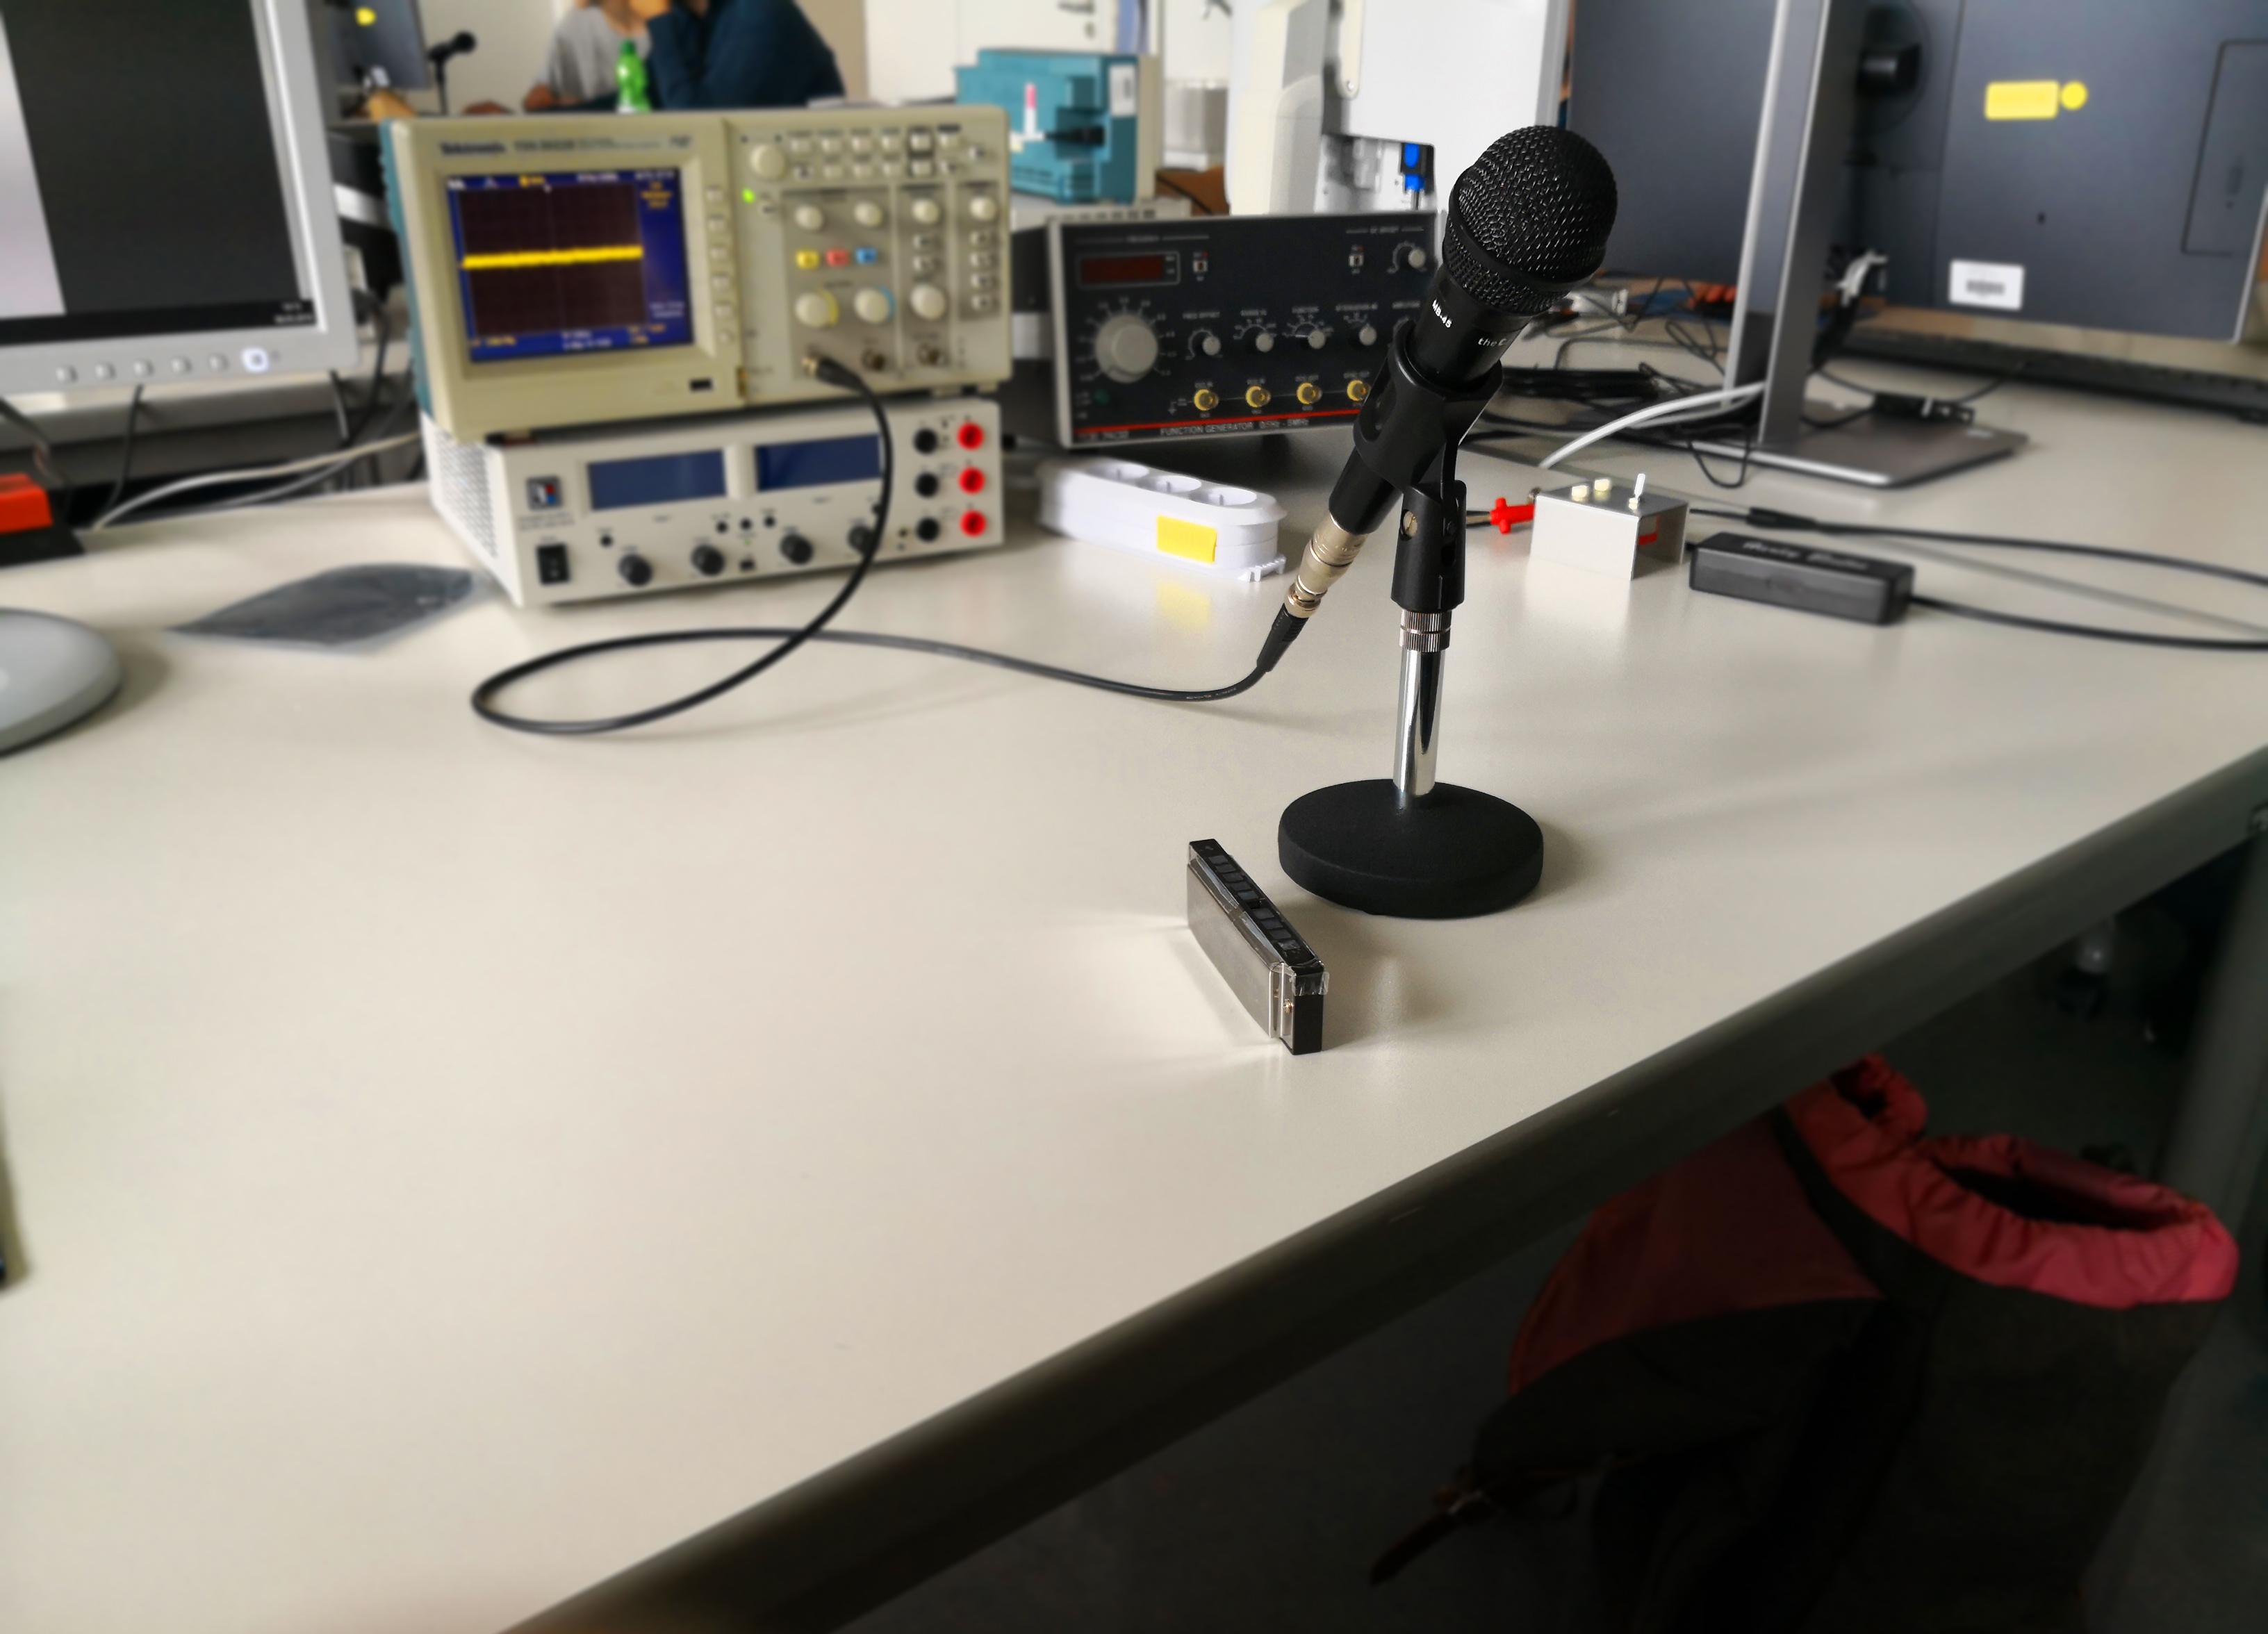
\includegraphics[width=0.8\textwidth]{media/aufbau2.jpg}
	\caption{Versuchsaufbau Teil 1}
	\label{img:Versuchsaufbau Teil 1}
\end{figure}
\newpage
Im Anschluss mussten wir mithilfe der Funktion numpy.fft.fft() die Fouriertransformation des Signals berechnen. Daraus sollten wir das Amplitudenspektrum bestimmen und graphisch darstellen.
Dabei ist zu beachten, dass die x-Achse mit der Frequenz nicht in Hertz sondern in der Anzahl Schwingungen innerhlab der gesamten Signaldauer definiert ist..
Die Frequenz f in Hertz lässt sich jedoch folgendermaße berechnen.
\\~\\
f = $\dfrac{n}{M * \Delta t}$
\\~\\
Als letzten Teil der ersten Aufgabe sollen wir die Grundfrequenz im Spektrum berechnen und damit die Frequenz in Hertz identifizieren.
Folgende Materialien wurden benötigt: ~\par
\begin{itemize}
	\item Oszilloskop
	\item Mikrofon
	\item Mundharmonika
	\item Signalkabel
	\item Python auf einem Computer
\end{itemize}
\newpage
\section{Messwerte}
\label{chap:VERSUCH_1_MESSWERTE}
Auf dem Bild ist das Signal abgebildet, dass wir mittels einer Mundharmonika in das Mikrofon geblasen haben.
\newline
Durch die Toolbox TekTDS2000 können wir das Signal nun in eine .csv Datei umwandeln und abspeichern.
\newline
Diese Datei haben wir mittels Numpy und der Funktion \textit{np.loadfromtxt} ausgelesen.
Die Ergebnisse wurden in die 2 verschiedene Funktionen x und y geschrieben.
\newline
Danach wurden diese mittels matplotlib graphisch dargestellt.
\begin{figure}[H]
	\centering\small
	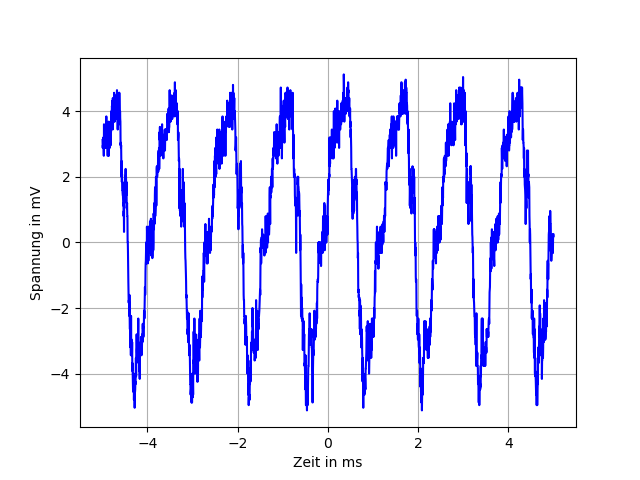
\includegraphics[width=0.9\textwidth]{../data/img/mundharmonika.png}
	\caption{Signal einer Mundharmonika}
	\label{img:Signal einer Mundharmonika}
\end{figure}
\newpage
\section{Auswertung}
\label{chap:VERSUCH_1_AUSWERTUNG}
Auf dem Spannungsverlauf sieht man das aufgenommene Signal der Mundharmonika.
Durch einen Pythonfunktion die wir aus der Toolbox TekTDS2000 erhalten haben, konnten wir den Spannungsverlauf aus dem Oszilloskop einlesen und in eine .csv Datei schreiben.
\newline
Dieses Format wird auch häufig für Excel Dateien verwendet.
Durch das Drücken des Knopfes Single Sequence haben wir auf dem Oszilloskop ein Standbild erhalten.
\newline
Diese Datei haben wir mittels Numpy und der Funktion \textit{np.loadfromtxt} ausgelesen.
Die Ergebnisse wurden in die 2 verschiedene Funktionen x und y geschrieben.
\newline
Danach wurden diese mittels matplotlib graphisch dargestellt.
\\~\\
Die Grundperiode und die Grundfrequenz haben wir uns mittels der Toolbox TekTDS2000 durch getFreq(1) und getPeriod(1) ausgeben lassen.
Die Signallänge M haben wir durch \textit{len(file.readlines())} erfahren.
\newline 
Durch die absolute Addition von den beiden Maxima- und Minimawerten erhalten wir gerundet die Signaldauer.
Wenn man nun die Signaldauer dividiert durch die Signallänge erhält man das Abtastintervall $\Delta$t mit dem Wert 4µs.
\newline
Mit dem Abtastintervall erhält man auch die Abtastfrequenz. Diese entspricht 250000  Hertz.
Im folgenden sind die Ergebnisse der Berechnungen aufzufinden:
\begin{table}[H]
	\centering\small
	\begin{tabular}{|c|c|}
	\hline
	Plot & Wert \\
	\hline
	Grundperiode (in ms) & 1.275ms \\
	\hline
	Grundfrequenz (in Hertz) & 784.31Hz \\
	\hline
	Signaldauer &  0,01s\\
	\hline
	Abtastfrequenz (in Kilohertz) &  250KHz\\
	\hline
	Signallänge M (Anzahl der Abtastzeitpunkte) & 2500 \\
	\hline
	Abtastintervall $\Delta$t (in µs) & 4µs \\
	\hline
	\end{tabular}
	\caption{Zu berechnende Werte}
	\label{fig:VERSUCH_1_MESSWERTE}
\end{table}
\newpage
Das Amplitudenspektrum erhält man indem man die Spannung absolut fouriertransformiert mit der Numpy Funktion \textit{np.fft.fft()} und als Amplitude auf der y Achse ausgibt. 
\newline
Doch bisher wird die x-Achse in der Einheit \textit{Anzahl Schwingungen innerhalb der gesamten Signaldauer} und nicht in Hertz angegeben. 
\newline
Um dies jedoch zu tun müssen wir die Frequenz in f folgendermaßen berechnen:
\\~\\
f = $\dfrac{n}{M * \Delta t}$
\\~\\
Die jeweilige Schwingung n wird geteilt durch die Signallänge und das Abtastintervall.
Dadurch erhält man folgenden Graphen, welcher bis zu dem von uns festgelegten Frequenzwert von 20000 geplotet wird.
\begin{figure}[H]
	\centering\small
	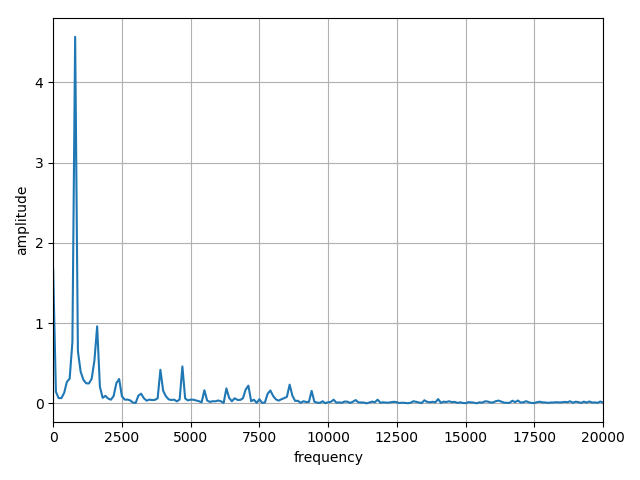
\includegraphics[width=0.8\textwidth]{../data/img/mundharmonika2.png}
	\caption{Das Amplitudenspekktrum von der Fourieranalyse}
	\label{img:Das Amplitudenspekktrum von der Fourieranalyse}
\end{figure}
\newpage
Mittels der Numpy Funktion \textit{np.max(spektrum)} können wir den maximalen Amplitudenwert abfragen.
Mittels einer for-Schleife fragen wir nun den Wert bis zum 1250sten Signal ab der das Maxima hat.
\newline 
Dadurch erhalten wir die Frequenz des maximalen Amplitudenwerts.
Wir fragen genau bis zur Hälfte der Werte ab, da der Graph sich spiegelt und es so 2 Maxima gibt. Da wir nur den ersten Wert wollen müssen wir dies festlegen.
\newline
Im folgenden sind die Ergebnisse der Berechnungen aufzufinden:
\begin{table}[H]
	\centering\small
	\begin{tabular}{|c|c|}
	\hline
	Plot & Wert \\
	\hline
	Maximaler Amplitudenwert & 4.5675 \\
	\hline
	Frequenz des Maxima & 800Hz \\
	\hline
	\end{tabular}
	\caption{Zu berechnende Werte}
	\label{fig:VERSUCH_1_MESSWERTE}
\end{table}
\newpage
\section{Interpretation}
\label{chap:VERSUCH_1_INTERPRETATION}
Da das Signal der Mundharmonika schön gleichmäßig ist, kann man feststellen, dass der Ton sehr gleichmäßig gespielt wurde. 
\newline 
Durch die Beschaffenheit des Funktionsweise und die laute Gegebenheiten zum Zeitpunkt der Messung, kann man gut beobachten, dass die Amplitude nach so gut wie jeder periodischen Wiederholung zunimmt und damit die Spannung auch höher wird.
Im großen Ganzen jedoch gibt es keine Unstimmigkeiten.
\\~\\
Für die Tabelle 2.1 kann man folgende Schlussfolgerungen ziehen: ~\par
\begin{itemize}
	\item Die Signaldauer ist komplementär mit der Signallänge und der dem Abtastintervall
	\item Das Abtastintervall ist komplementär zur Abtastfrequenz
	\item Frequenz und Zeit sind komplementär zueinander
\end{itemize}
\\~\\
Bei der Abbildung 2.3 ist eine schöne Amplitude zu erkennen, die sich von den anderen Amplituden durch ihre Höhe absetzt.
Dieser maximale Amplitudenausschlag mit der Höhe 4.5675V ist der Ton.
\newline 
Der Ton den wir produziert haben liegt also demnach bei 800Hz. Da wir bis auf eine Öffnung die Anderen zugeklebt haben, wissen wir dass wir einen Ton mit der Frequenz von 800Hz gespielt haben. 
\newline
Die anderen kleinen Harmonischen sind die Obertöne.
Wir wissen durch das Amplitudenspektrum auch, dass wir keinen Klang gespielt haben und die Mundharmonika richtig zugeklebt haben.
\\~\\
Wenn man die Fouriertransformierte für alle 2500 Abtastungen graphisch darstellt, dann stellt sich eine y-Achsenspiegelung dar.
Da wir jedoch keine Achsenspiegelung wollen sondern ledigliche bis Frequenzen von 20000Hz kürzen wir die x-Achse um nur die wichtigen Werte zu erlangen.
%
% CHAPTER Versuch 2
%
\chapter{Versuch 2}
\label{chap:VERSUCH_2}
\section{Fragestellung, Messprinzip, Aufbau, Messmittel}
\label{chap:VERSUCH_2_FRAGESTELLUNG}
In dem zweiten Versuch war es die Aufgabe für jeden der beiden Lautsprecher die Amplitude und die Phasenverschiebung des akustischen Ausgangssignales zu ermitteln, indem man sowohl die Eingangs- als auch das Mikrofonsignal auf dem Oszilloskop darstellt.
\newline 
Eines der beiden Diagramme haben wir abgespeichert welches in der Abbildung 3.1 einsehbar ist.
Zudem berechnen wir jeden der 17 verschiedenen Frequenzen für jeweils den großen und den kleinen Lautsprecher die Amplitude und die Phasenverschiebung.
Die 17 verschiedenen Frequenzen sind folgende:
\newline
100Hz, 200Hz, 300Hz, 400Hz, 500Hz, 700Hz, 850Hz, 1000Hz, 1200Hz, 1500Hz, 1700Hz, 2000Hz, 3000Hz, 4000Hz, 5000Hz, 6000Hz, 10000Hz
\end{itemize}
\\~\\
Diese geben wir im Laufe des Versuches in einer Tabelle aus.
Wichtig ist es hierbei bei beiden Lautsprechern den selben Abstand zu haben. Zudem sollten beide Kanäle auf AC Coupling gestellt sein, da wir den Gleichanteil nicht benötigen.
\newline
Wie bei dem ersten Versuch verwenden wir wieder den Single Sequence Mode um ein Standbild des Signals zu erhalten um dieses besser zu capturen.
\newline
Nach der Aufnahme des Signals ist es wichtig für die nächste Frequenz wieder den Single Sequence Mode zu deaktivieren um ein neues Bild zu erhalten.
\\~\\
Das Eingangssignal soll konstant auf 1.5V eingestellt sein. Mit jeder Veränderung der Frequenz muss die Amplitude wieder angepasst werden.
Danach sollen wir die Daten der Amplitude und der Phasenverschiebung in Arrays transferieren und graphisch darstellen.
\newpage
Für beide Lautsprecher werden wir mit matplotlib ein Bode-Diagramm darstellen, indem wir beide Diagramme mit der Funktion semilogx() halblogarithmisch darstellen und den Phasenwinkel dazu berechnen mit der Formel:
\\~\\
Amplitude = 1 / Amplitude
\newline
Amplitude = 20$\log _{10}$ * Amplitude
\\~\\
Phasenwinkel = -$\Delta$t * f * 360
\\~\\
\begin{figure}[H]
	\centering\small
	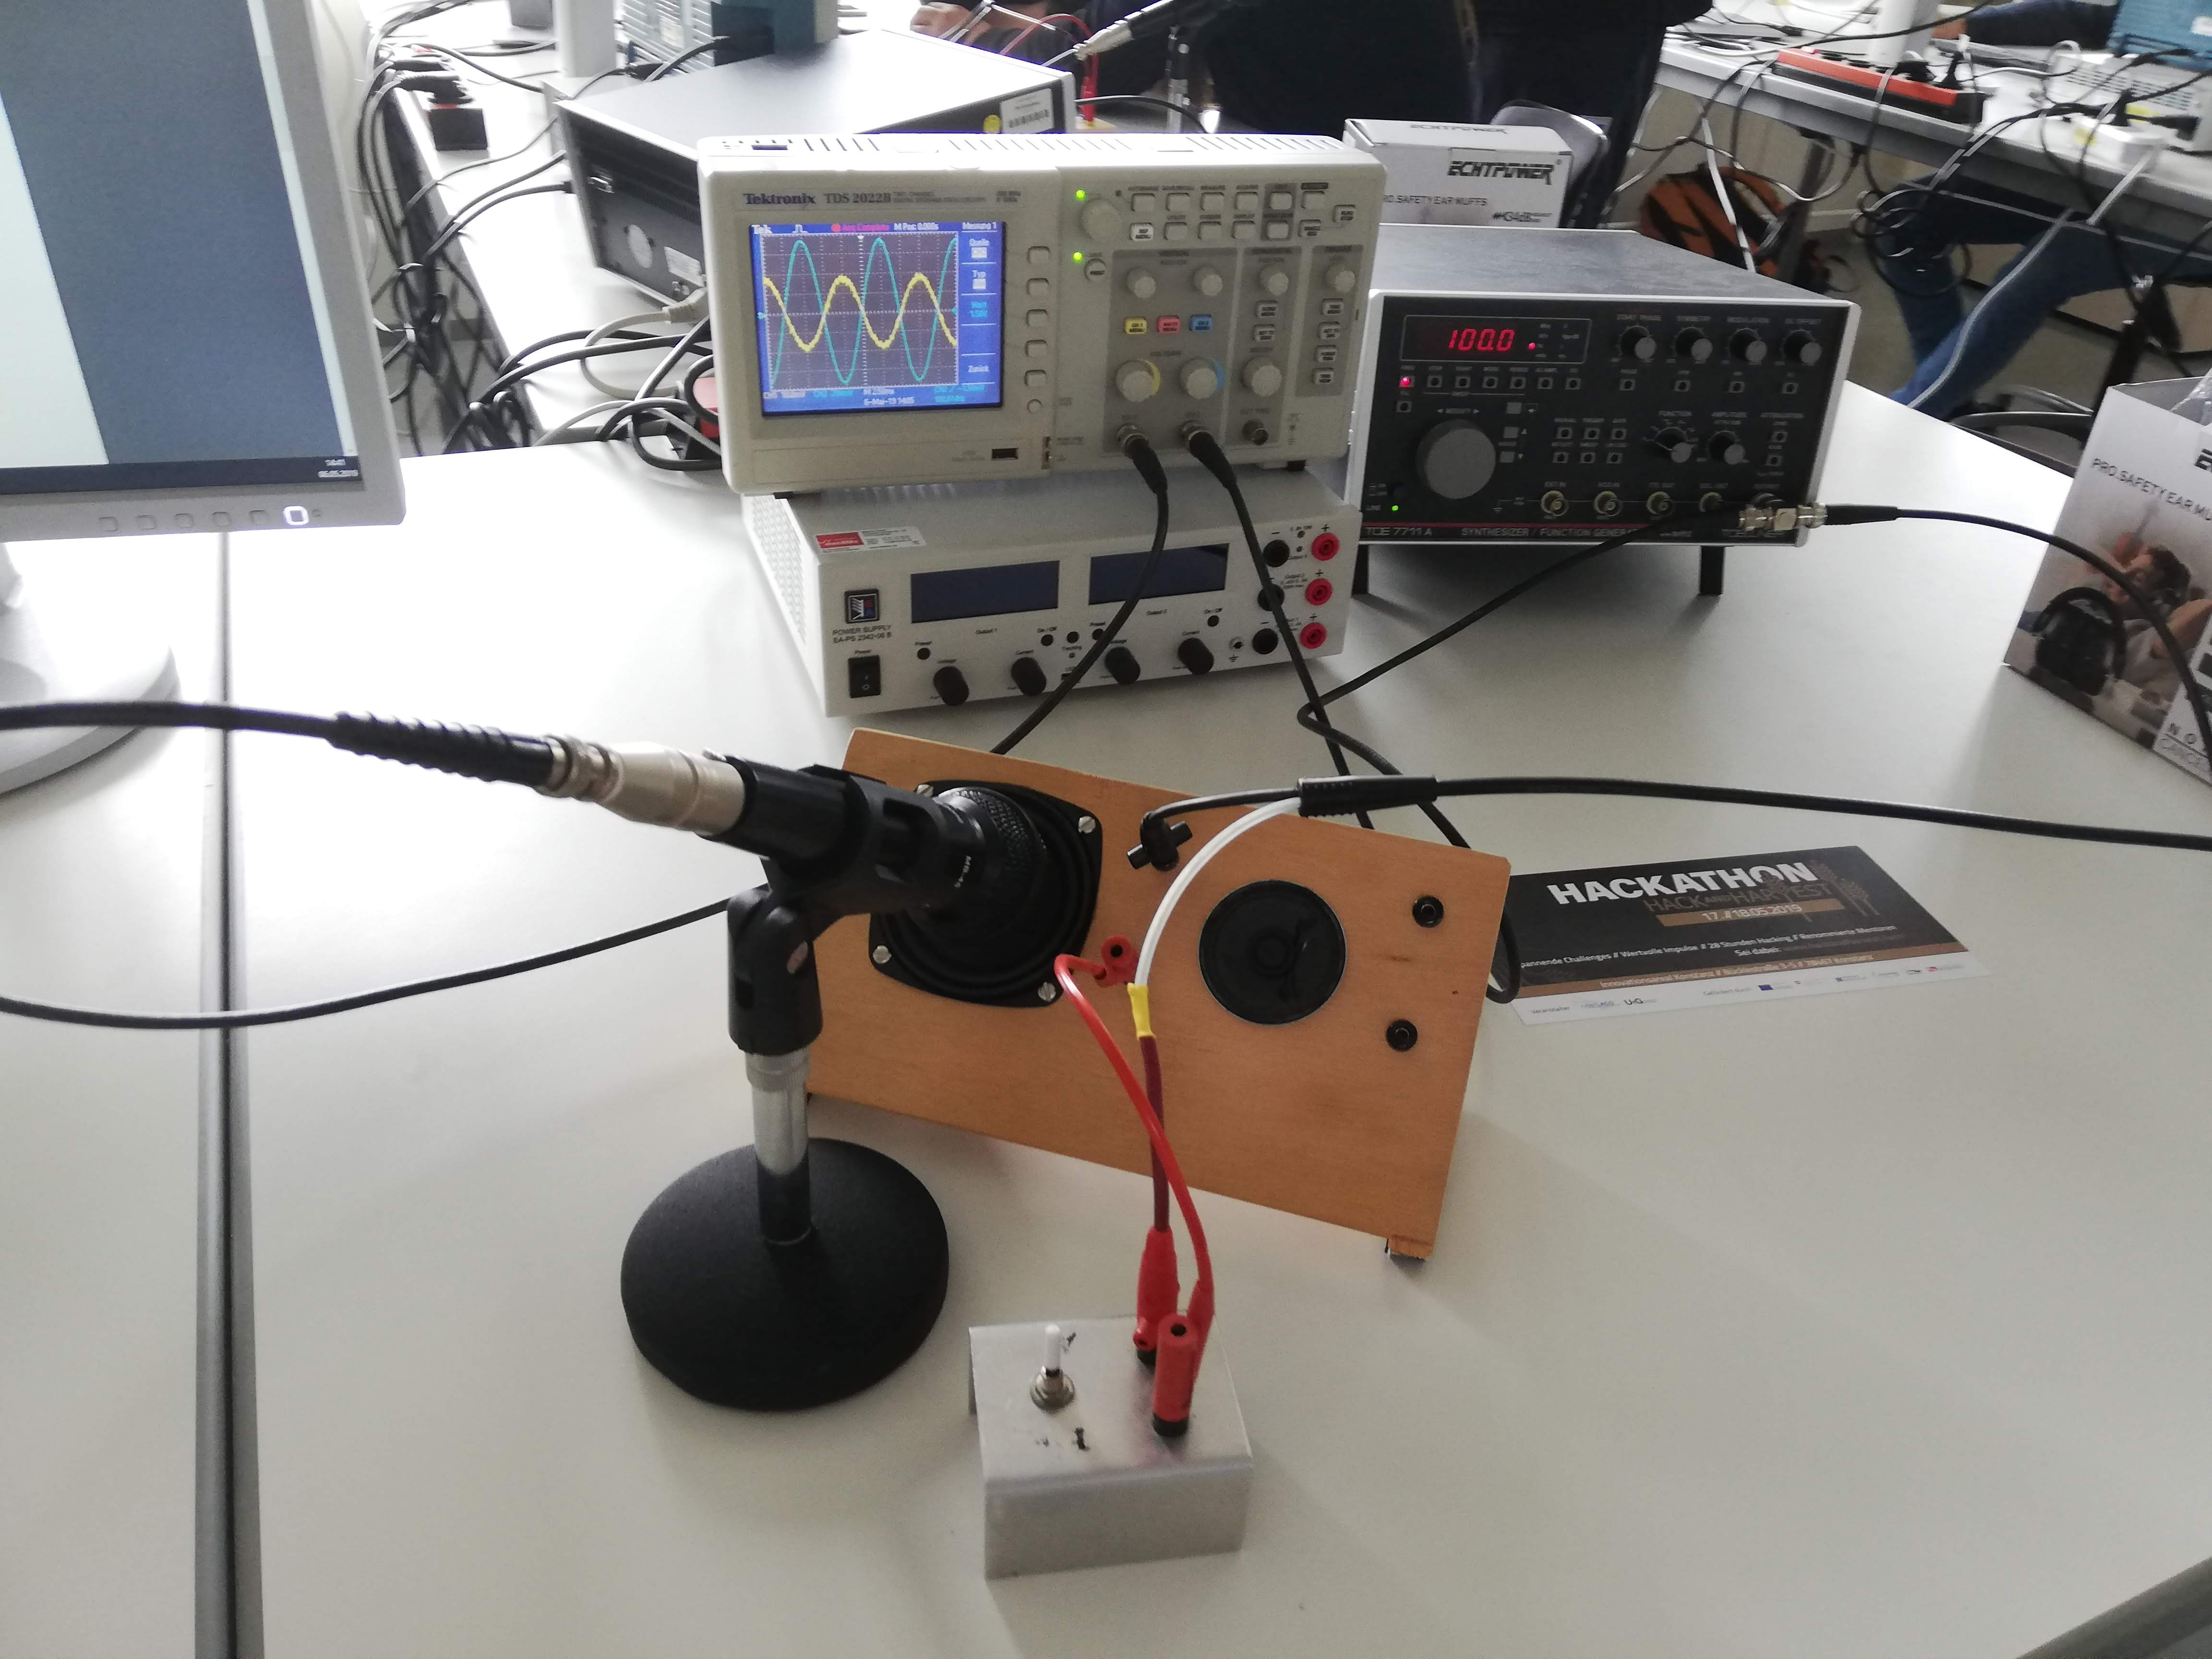
\includegraphics[width=0.9\textwidth]{media/aufbau.jpg}
	\caption{Signal einer Mundharmonika}
	\label{img:Signal einer Mundharmonika}
\end{figure}
\newpage
In dem zweiten Versuch schließen wir das Mikrofon erneut an den Channel 1 des Oszilloskopes. Der Lautsprecher wird mit dem Pluspol an den An- und Ausschalter angeschlossen.
Der Schalter wiederrum wird wiederrum mit dem Negativkabel verbunden und in den Verstärker geleitet. 
\newline
Den Schalter benötigen wir, um den nervtötenden Ton direkt wieder zu eliminieren, sobald man eine Single Sequence besitzt. Der Verstärker wiederrum geht in den Channel 2 des Oszilloskopes. 
Der Verstärker wird wiederrum an den Output des Oszilloskopes angehängt.
\newline
Der Abstand vom Mikrofon zum Lautsprecher soll bei beiden Lautsprechern gleich sein.
\\~\\
Folgende Materialien wurden benötigt: ~\par
\begin{itemize}
	\item Oszilloskop
	\item Verstärker
	\item 2 verschiedene Lautsprecher
	\item Schalter 
	\item Mikrofon
	\item Mundharmonika
	\item Signalkabel Schwarz
	\item Signalkabel Rot
	\item Signalkabel, dass Plus mit Minus verbindet und beide weiterleitet
	\item Adapter für Verstärker
	\item Python auf einem Computer
\end{itemize}
\newpage
\section{Messwerte}
\label{chap:VERSUCH_2_MESSWERTE}
Auf der linken Seite ist die Single Sequence des Oszilloskopes bei einer Frequenz von 100Hz. Dabei stellt das gelbe Signal den Input beziehungsweise das Mikrofon dar, während das blaue Signal vom Channel 2 stammt und der Output für den Lautsprecher ist.
Bei beiden Signalen sehen wir eine gleichmäßige Sinuskurve. Die beiden Signale wurden in .csv Dateien gespeichert. Der Input von Channel 1 wurde dabei nochmals von uns eingelesen in einem Pythonskript und wurde daraufhin graphisch ausgegeben.
\begin{figure}[H]
\centering
\begin{subfigure}{.5\textwidth}
  \centering
  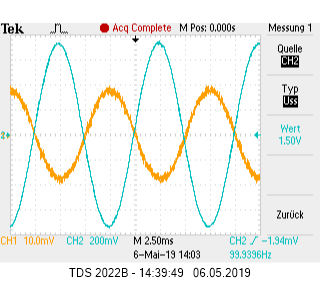
\includegraphics[width=0.9\linewidth]{../data/img/100.png}
  \caption{Die Ausgabe des Oszilloskopes}
  \label{fig:Die Ausgabe des Oszilloskopes}
\end{subfigure}%
\begin{subfigure}{.5\textwidth}
  \centering
  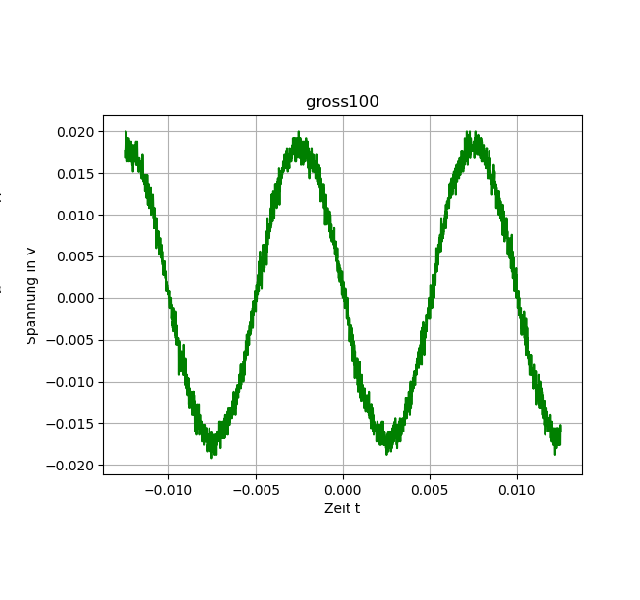
\includegraphics[width=0.9\linewidth]{../data/img/gross100.png}
  \caption{Die Auswertung der .csv Datei durch Python}
  \label{fig:Die Auswertung der .csv Datei durch Python}
\end{subfigure}
\caption{Einlesen des Signals durch das Oszilloskop und in die .csv Datei}
\label{fig:Einlesen des Signals durch das Oszilloskop und in die .csv Datei}
\end{figure}
Wir haben für jede Frequenz und sowohl für Input als auch Output jeweils eine graphische Darstellung.
Da diese jedoch den Rahmen sprengen würde und zudem das Dokument viel zu unübersichtlich wäre, reduziere ich die Darstellung auf die Frequenz von 200Hz.
\newpage
In der Abbildung 3.3 haben wir die abgebildete Rückkopplung für den kleinen und den großen Lautsprecher bei jeweils 200Hz.
Links ist der kleine Lautsprecher abgebildet und rechts der große Lautsprecher.
\begin{figure}[H]
\centering
\begin{subfigure}{.5\textwidth}
  \centering
  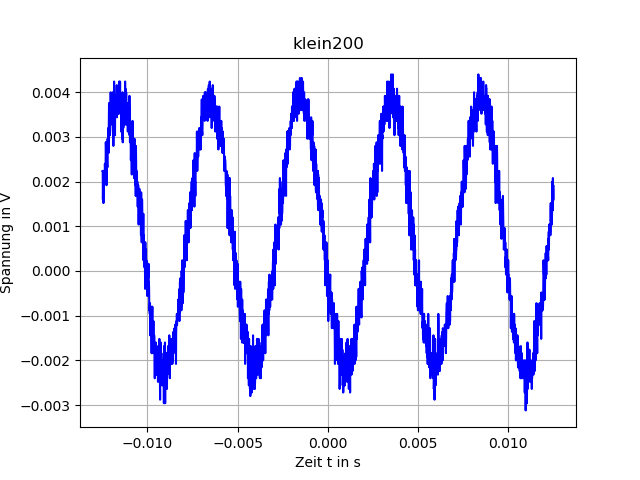
\includegraphics[width=0.9\linewidth]{../data/img/klein200.png}
  \caption{Die Spannung bei dem kleinen Lautsprecher und einer Frequenz von 200Hz}
  \label{fig:Die Spannung bei dem kleinen Lautsprecher und einer Frequenz von 200Hz}
\end{subfigure}%
\begin{subfigure}{.5\textwidth}
  \centering
  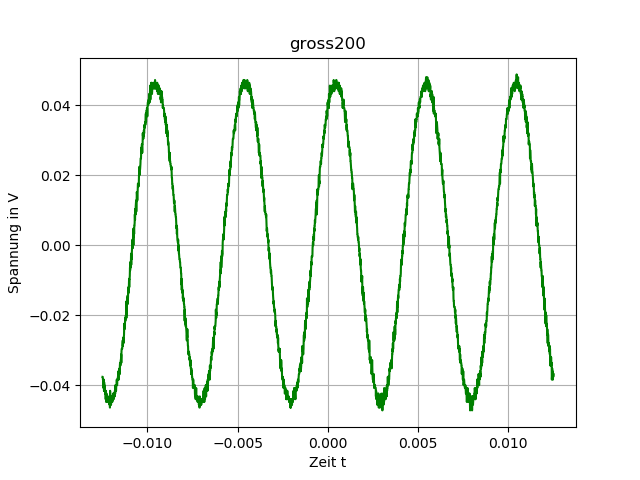
\includegraphics[width=0.9\linewidth]{../data/img/gross200.png}
  \caption{Die Spannung bei dem großen Lautsprecher und einer Frequenz von 200Hz}
  \label{fig:Die Spannung bei dem großen Lautsprecher und einer Frequenz von 200Hz}
\end{subfigure}
\caption{Vergleich zwischen dem kleinen und dem großen Lautsprecher bei einer Frequenz von 200Hz}
\label{fig:Vergleich zwischen dem kleinen und dem großen Lautsprecher bei einer Frequenz von 200Hz}
\end{figure}
\newpage
\section{Auswertung}
\label{chap:VERSUCH_2_AUSWERTUNG}
Auf dem Spannungsverlauf beziehungsweise den Spannungsverläufen sieht man die Spannung die bei einer Rückkopplung entsteht bei bestimmten Frequenzen. Diese wurden auf dem Oszilloskop angezeigt und durch ein von uns mithilfe der Toolbox TekTDS2000 erstelltes Pythonskript in eine .csv Datei geschrieben.
\newline 
Dabei haben wir jeweils eine .csv Datei erstellt für Channel 1 (Mikrofon als Input) und für Channel 2 (Lautsprecher als Output).
Die .csv Dateien werden von uns in einem Pythonskript wieder eingelesen und die Werte in Arrays gespeichert. 
\newline 
Aus den Daten stellen wir wiederrum die Amplitude und den Phasengang graphisch dar.
\\~\\
Mit der Numpy Funktion \textit{np.max(np.abs())} erhalten wir den maximalen absoluten Wert des Signals beziehungsweise die Amplitude.
Dies machen wir mit sämtlichen 17 unterschiedlichen Frequenzen.
Das Signal das gelb abgebildet ist, beschreibt die Amplitude des großen Lautsprechers, während das blaue Signal die Amplitude des kleinen Lautsprechers darstellt.
Daraus erhalten wir die folgenden graphischen Darstellungen.
\begin{figure}[H]
\centering
\begin{subfigure}{.5\textwidth}
  \centering
  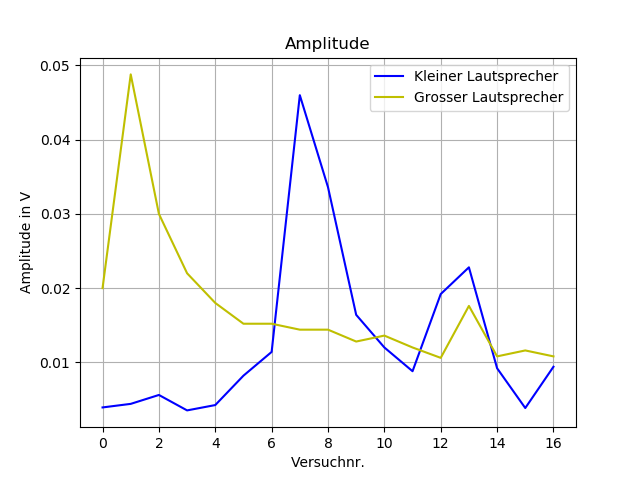
\includegraphics[width=0.9\linewidth]{../data/img/amplitudeanzahl.png}
  \caption{Amplitude mit der zugehörigen Dateinummer}
  \label{fig:Amplitude mit der zugehörigen Dateinummer}
\end{subfigure}%
\begin{subfigure}{.5\textwidth}
  \centering
  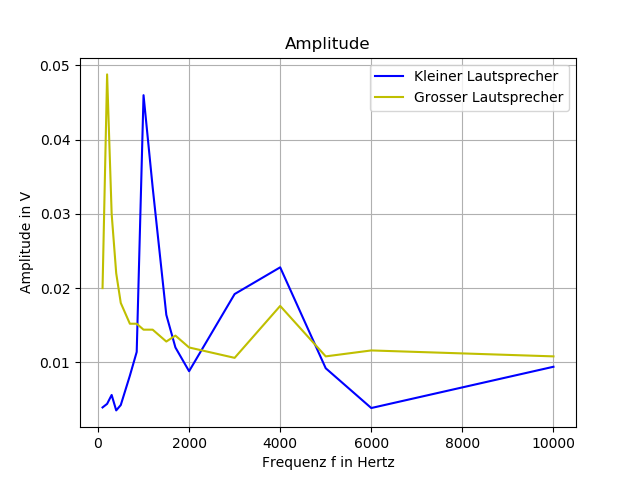
\includegraphics[width=0.9\linewidth]{../data/img/amplitudefrequenz.png}
  \caption{Amplitude mit der zugehörigen Frequenz}
  \label{fig:Amplitude mit der zugehörigen Frequenz}
\end{subfigure}
\caption{Amplitude mit Dateinummmer und zugehöriger Frequenz}
\label{fig:Amplitude mit Dateinummmer und zugehöriger Frequenz}
\end{figure}

\newpage

Die Phasenverschiebung zu berechnen ist etwas komplizierter als erst gedacht.
Zuerst schauen wir uns den Plot an der uns für die jeweiligen Frequenzen ausgegeben wird.


\begin{figure}[H]
	\centering\small
	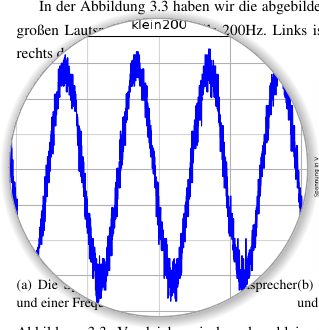
\includegraphics[width=0.4\textwidth]{media/phase.png}
	\caption{Beispiel einer Phasenverschiebung}
	\label{img:Beispiel einer Phasenverschiebung}
\end{figure}

Der Achsenschnittpunkt befindet sich in der Mitte. Dort sollte also auch der Anfang der Sinuskurve sein. Da der Abstand zum nächsten Nullpunkt auf der rechten Seite des Achsenschnittpunktes ist, müssen wir nun in der .csv Tabelle den nächsten Nullpunkt finden.
Der Achsenschnittpunkt liegt bei der Zeile 1250. Deshalb müssen wir nun tiefer suchen nach einem Nullpunkt.

\begin{figure}[H]
	\centering\small
	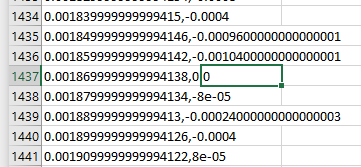
\includegraphics[width=0.7\textwidth]{media/excel.png}
	\caption{Phasenverschiebung in einer .csv Datei}
	\label{img:Phasenverschiebung in einer .csv Datei}
\end{figure}
\newpage
Hier haben wir den Nullpunkt in der Zeile 1437. Deshalb rechnen wir nun 1437 - 1250 = 187 Signallänge
Die Singallänge von 87 multiplizieren wir nun mit dem Abtastintervall. Das Abtastintervall erhalten wir durch die Subtraktion zweier benachbarter Werte, die daraufhin auf 5 Nachkommastellen gerundet werden.
\\~\\
\textit{187 Signallänge *  1 µs  = 187 µs} 
\\~\\
Nun haben wir die Phasenverschiebung berechnet. An dem Beispiel für den kleinen Lautsprecher mit einer Frequenz von 200Hz beträgt die Phasenverschiebung also 187Hz.
Nachdem wir sämtliche Phasenverschiebungen berechnet haben, geben wir diese graphisch in einem Plot wieder.
Das gelbe Signal ist erneut der große Lautsprecher, während das blaue Signal der kleine Lautsprecher ist.
Im linken Bild ist der Phasengang in Abhängigkeit zur Dateinummer und im rechten Bild ist der Phasengang in der Abhängigkeit zur Frequenz.
\begin{figure}[H]
\centering
\begin{subfigure}{.5\textwidth}
  \centering
  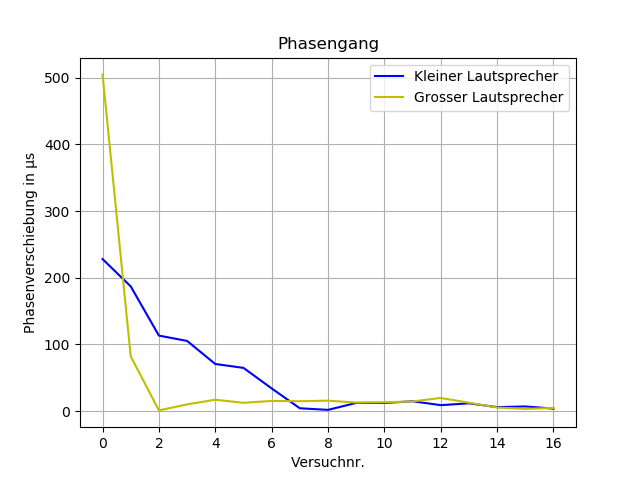
\includegraphics[width=0.9\linewidth]{../data/img/phasenanzahl.png}
  \caption{Phasengang mit der zugehörigen Dateinummer}
  \label{fig:Phasengang mit der zugehörigen Dateinummer}
\end{subfigure}%
\begin{subfigure}{.5\textwidth}
  \centering
  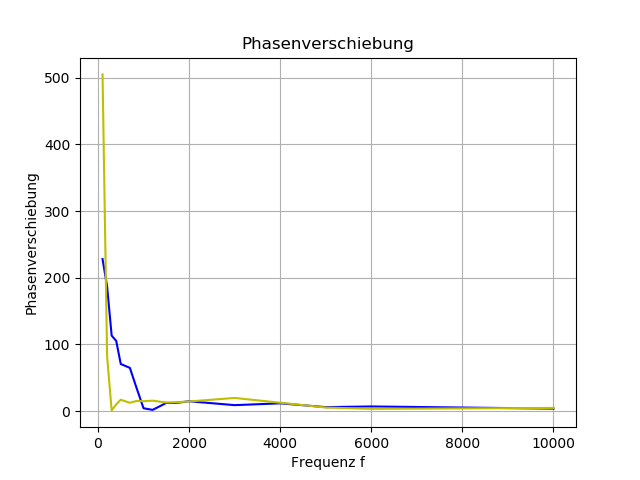
\includegraphics[width=0.9\linewidth]{../data/img/phasenfrequenz.png}
  \caption{Phasengang mit der zugehörigen Dateinummer}
  \label{fig:Phasengang mit der zugehörigen Dateinummer}
\end{subfigure}
\caption{Phasengang mit der zugehörigen Frequenz}
\label{fig:Phasengang mit der zugehörigen Frequenz}
\end{figure}
\newpage
Das Bode Diagramm für die Amplitude wird folgendermaßen berechnet:
\\~\\
\textit{amplitude = 1 / amplitude} 
\newline
\textit{amplitude = 20 * $\log_{10} amplitude$} 
\\~\\
Nun muss man nur noch bei sämtlichen plots die Numpy Funktion np.semilogx() anwenden um die Diagramme halblogarithmisch dazustellen.
\begin{figure}[H]
\centering
\begin{subfigure}{.5\textwidth}
  \centering
  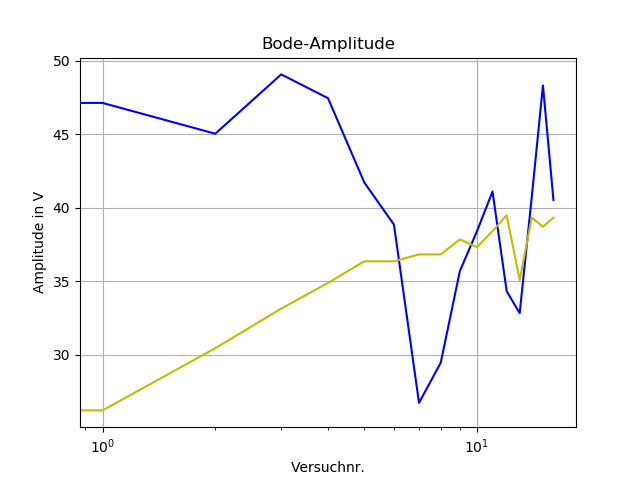
\includegraphics[width=0.9\linewidth]{../data/img/bodeamplitudeanzahl.png}
  \caption{Bode-Diagramm für die Amplitude mit Dateinummer}
  \label{fig:Bode-Diagramm für die Amplitude mit Dateinummer}
\end{subfigure}%
\begin{subfigure}{.5\textwidth}
  \centering
  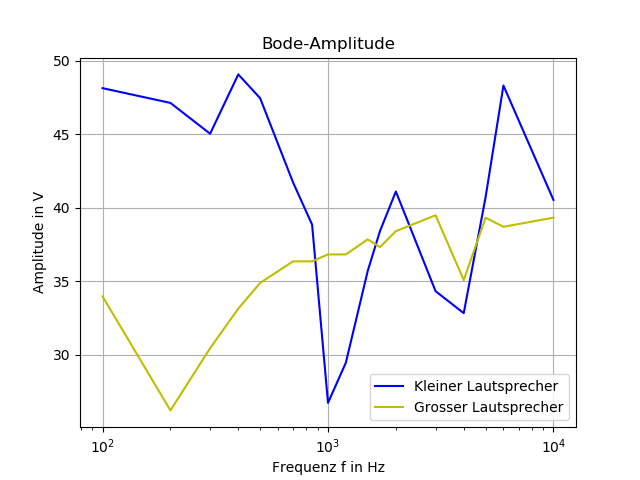
\includegraphics[width=0.9\linewidth]{../data/img/bodeamplitudefrequenz.png}
  \caption{Bode-Diagramm für die Amplitude mit Frequenz}
  \label{fig:Bode-Diagramm für die Amplitude mit Frequenz}
\end{subfigure}
\caption{Bode Diagramm für die Frequenz}
\label{fig:Bode Diagramm für die Frequenz}
\end{figure}
\newpage
Das Bode Diagramm für die Phasenverschiebung wird folgendermaßen berechnet:
\\~\\
\textit{Phasenwinkel = -$\Delta$t * f * 360} 
\\~\\
Nun muss man nur noch bei sämtlichen plots die Numpy Funktion np.semilogx() anwenden um die Diagramme halblogarithmisch dazustellen.
\begin{figure}[H]
\centering
\begin{subfigure}{.5\textwidth}
  \centering
  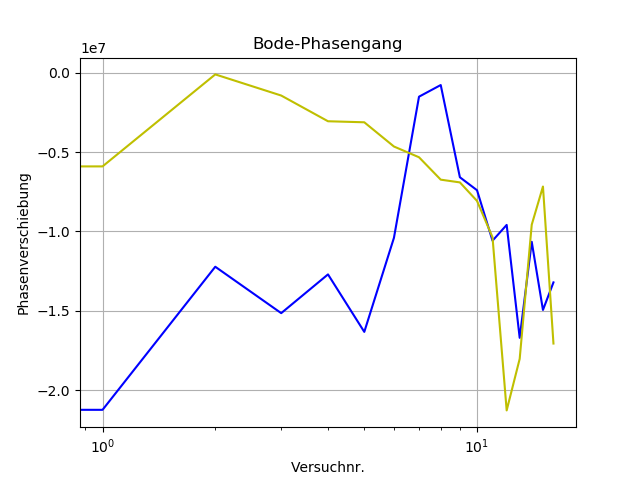
\includegraphics[width=0.9\linewidth]{../data/img/bodephasenanzahl.png}
  \caption{Bode-Diagramm für den Phasengang mit Dateinummer}
  \label{fig:Bode-Diagramm fürden Phasengang mit Dateinummer}
\end{subfigure}%
\begin{subfigure}{.5\textwidth}
  \centering
  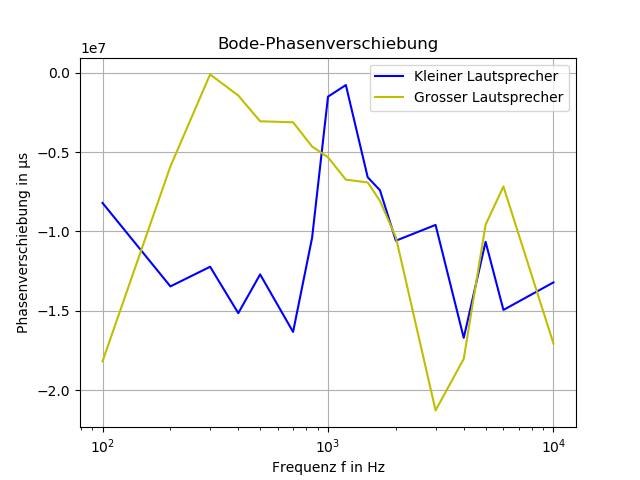
\includegraphics[width=0.9\linewidth]{../data/img/bodephasenfrequenz.png}
  \caption{Bode-Diagramm für den Phasengang mit Frequenz}
  \label{fig:Bode-Diagramm für den Phasengang mit Frequenz}
\end{subfigure}
\caption{Bode-Diagramm für den Phasengang}
\label{fig:Bode-Diagramm für den Phasengang}
\end{figure}

\newpage
\section{Interpretation}
\label{chap:VERSUCH_2_INTERPRETATION}
In der Abbildung 3.3 kann man die gut die Unterschiede zwischen dem kleinen und dem großen Lautsprecher erkennen.
Der kleine Lautsprecher hat ein sehr ungenaues und unfeines Signal. 
\newline
Der große Lautsprecher hingegen hat klare Linien und Kurven.
Das lässt darauf deuten, dass der große Lautsprecher mehr Watt hat und seinen Output klarer an das Mikrofon weitergeben konnte.
\newline
Damit lässt sich beweisen, dass der große Lautsprecher qualitativ besser ist.
\\~\\
In dem linken Schaubild in der Abbildung 3.7 divergiert die Phasenverschiebung mit zunehmender Frequenz immer mehr Richtung 0.
\newline
Da das Mikrofon Frequenzen von 70Hz bis 13KHz aufnehmen kann, stellen die von uns gemessenen Frequenzen keine Probleme dar in unseren Abbildungen.
\\~\\

%
% CHAPTER Anhang
%
\renewcommand\thesection{A.\arabic{section}}
\renewcommand\thesubsection{\thesection.\arabic{subsection}}

\chapter*{Anhang}
\label{chap:APPENDIX}
\addcontentsline{toc}{chapter}{Anhang}
%\setcounter{chapter}{0}
\addtocounter{chapter}{1}
\setcounter{section}{0}

\section{Quellcode}
\label{chap:APPENDIX_SOURCECODE}

\subsection{Quellcode Versuch 1.1}
\label{chap:APPENDIX_SOURCECODE_V1.1}
\lstinputlisting[style=PYTHON, frame=single, caption=Das Bild des Oszilloskopes einlesen und abspeichern, captionpos=b, label=lst:APPENDIX_SOURCECODE_AREA1]{../task1.1.py}
\newpage
\subsection{Quellcode Versuch 1.2}
\label{chap:APPENDIX_SOURCECODE_V1.2}
\lstinputlisting[style=PYTHON, frame=single, caption=.csv Datei einlesen und in einem Plot graphisch wiedergeben, captionpos=b, label=lst:APPENDIX_SOURCECODE_AREA1]{../task1.2.py}
\subsection{Quellcode Versuch 1.3}
\label{chap:APPENDIX_SOURCECODE_V1.3}
\lstinputlisting[style=PYTHON, frame=single, caption=Fouriertransformation anwenden und ein Amplitudenspektrum ausgeben  sowie Berechnung einiger Werte, captionpos=b, label=lst:APPENDIX_SOURCECODE_AREA1]{../task1.3.py}
\newpage
\subsection{Quellcode Versuch 2.1}
\label{chap:APPENDIX_SOURCECODE_V2.1}
\lstinputlisting[style=PYTHON, frame=single, caption=Lautsprecherdaten graphisch ausgeben und einige Werte berechnen, captionpos=b, label=lst:APPENDIX_SOURCECODE_AREA1]{../task2.1.py}
\newpage
\subsection{Quellcode Versuch 2.2}
\label{chap:APPENDIX_SOURCECODE_V2.2}
\lstinputlisting[style=PYTHON, frame=single, caption=Amplitude\, Phasenverschiebung und Bode-Diagramm berechnen, captionpos=b, label=lst:APPENDIX_SOURCECODE_AREA1]{../task2.2.py}
\newpage
\section{Messergebnisse}
\label{chap:APPENDIX_MEASUREMENT_SOURCE}
\begin{figure}[H]
	\centering\small
	\includegraphics[width=0.9\textwidth]{media/mess.png}
	\caption{Messergebnisse für Task 2}
	\label{img:Messergebnisse für Task 2}
\end{figure}
%
% Literaturverzeichnis
%
%
% Literaturverzeichnis
%
\phantomsection
\addcontentsline{toc}{chapter}{Literaturverzeichnis}
\bibliography{../references}
\newpage

\end{document}
%------------------------------------
% ╔═╗╔╗╔╔╦╗  ╔╦╗╔═╗╔═╗╦ ╦╔╦╗╔═╗╔╗╔╔╦╗
% ║╣ ║║║ ║║   ║║║ ║║  ║ ║║║║║╣ ║║║ ║ 
% ╚═╝╝╚╝═╩╝  ═╩╝╚═╝╚═╝╚═╝╩ ╩╚═╝╝╚╝ ╩ 
%------------------------------------